\chapter{Mixture processing models} 

\label{Chapter 5}

\lhead{Chapter 5. \emph{Mixture models}}
\vspace{3cm}
\newpage

% New Sections for Ami to read
% - Sections highlighted in red in intro and discussion. 
% - I replaced the introductory proofs with a Figure to illustrate how channel RTs were combined to produce the canonical models (your suggestion from earlier this year, I think it works.)

%%AE: please make sure the figures are in good shape Paul, some ( 5.5, 5.6, 5.7, 5.8; perhaps others?) seems to be very low res, which makes them hard to see
%PG: Yep, this has now been fixed. Not sure what caused that.

\noindent
The results of this Chapter appear in the published manuscript `Systems factorial technology analysis of mixtures of processing architectures' \cite{Little2018mixmodel}.

\section{Chapter overview}
In a complex and ever changing environment, people must often process information from multiple sources. In previous Chapters, we have described how information processing systems may be diagnosed by several key attributes using SFT \cite{Townsend_1995, Townsend_2004, Little2017}. These attributes include the architecture (parallel vs serial), stopping-rule (exhaustive vs self-terminating), workload capacity (limited, unlimited, or super), and (in)dependence of the processing channels (facilitatory, independent, or inhibitory). SFT allows the identification of qualitatively different patterns of information processing models based on non-parametric analysis of response-time data. The purpose of this Chapter is to extend the application of SFT to those cases where there is a probabilistic mixture of two qualitatively different processing architectures. 

Humans display remarkable flexibility in how we combine and process information. For example, as we contemplate everyday situations, we can shift our attention to `low-level' perceptual or `high-level' conceptual aspects of a scene, (\eg a set of red items vs a vine of tomatoes), retrieve memories of an experience, (\eg numerical value `AND' guests for dinner tonight), and integrate these source to make a decision, (\eg I will need six of these tomatoes for dinner tonight). The integration of these different processes implies that, rarely, a processing system would purely reflect a singular set of attributes, (\eg entirely parallel or entirely serial). Mixtures of different processing models are likely to describe many everyday decisions, including categorization \cite{Little2011, Moneer2016, Cheng2017, Griffiths2017}, visual working memory \cite{Donkin2013}, controlled vs automatic processing \cite{Shiffrin1977,schneider1977controlled}, and comparative numerosity.

In the previous Chapter, we considered the possibility that response-times might reflect a mixture of two processing architectures. These mixtures may occur when different processing architectures are used on different trials of an experiment. For example, within numerical comparisons, a serial processing architecture may be adopted when quantities are near a criterion and workload is high, yet, when quantities are far from the criterion, processing architecture may switch to parallel. Similarly, mixtures of processing architecture may occur when channels move from being dependant, to independent, (\eg coactive to parallel). In the previous Chapter, we provided two example of such mixtures, however, examples also exist in other realms of cognition. For example, accessing memories might occur through the coactive pooling of information; yet, the decisional process may occur via independent-channels, in either parallel or serial.

Mixtures of processing architecture may describe many cognitive processes, yet, the signatures of these models have not been identified for the survivor interaction contrast and capacity coefficient. In this Chapter, we will generate and report SFT predictions for model mixtures, (\eg parallel vs serial), using the SIC($t$) and capacity coefficient. We will systematically vary the relative proportions of each component model, and visualize these mixtures with our distributional response-time measures. As the reader will soon see, results from these mixture models are different from those typically found using canonical or `pure' processing models and in some instances, reflect those mixtures reported in the discussion of Chapter \ref{Chapter 4}.

\section{Response-time mixtures}
The time taken to make a decision reflects a mixture of cognitive processes. For example, \citeA{luce1963detection} characterized a decision as the combination of external information and internal biases; whereas \citeA{Falmagne1965} characterised fast and slow responses as the mixture of preparatory and reactionary states, (\ie proactive and reactive control; \citeauthor{braver2007}, 2007). These accounts describe how cognitive processes mix, and the impact such mixtures have on decision response-times; yet, provide no insight into the mixture of processing systems --- how information channels mix and the effect this has on RT. 

Processing system mixture models have been of interest to the SFT community. In a recent special issue on SFT, \citeA{TillmanStopping} assessed how the SIC changed over mixtures of system stopping-rule (exhaustive vs self-terminating), within parallel and serial processing architectures. They observed smooth changes in canonical form, as relative mixture proportions shifted in favor of one processing model to another (Figures 1--2 of their paper). However, this investigation was limited to those instances where processing channels did not interact. Prior to this study, \citeA{eidels2011} investigated parallel models that allowed interactions across processing channels. Using both the SIC and capacity coefficient, \citeA{eidels2011} showed smooth changes in canonical form, from parallel facilitatory (coactive) channels, to parallel inhibitory channels (Figure 3 of their paper). 

The current Chapter will extend the work of both \citeA{TillmanStopping} and \citeA{eidels2011}. Here, we consider the impact of mixture models when processing architecture moves from parallel to serial, and when processing channels move from independent to facilitatory \cite<à la>{eidels2011}. As processing architecture and workload capacity are closely related, we will visualise these mixtures using both the SIC and capacity coefficient. Given the insights of \citeA{TillmanStopping}, the current work will be restricted to those cases where stopping-rule does not change.

Restricting our investigation to mixtures of processing architecture, and not mixtures of stopping-rule, makes sense under experimental settings. When a task requires the exhaustive processing of two information-sources, (\eg where channel A `AND' channel B must be a target), a self-terminating stopping-rule becomes a liability. Similarly, when a task requires only a single-target in either location, (\eg where channel A `OR' channel B must be a target), an exhaustive stopping-rule becomes non-strategic. In the SFT literature, we term these `AND' and `OR' tasks respectively. Importantly, these task-types are always tested independently, either in separate blocks or separate experiments. As such, from trial-to-trial, it is unlikely that stopping-rule would change when the task-requirements are always exhaustive, or always self-terminating. 

\section{AND vs OR capacity}
Assessing the system architecture and workload capacity of AND and OR tasks has been a key contribution of SFT. Measures of processing architecture --- the MIC and SIC --- are equally applicable regardless of task stopping-rule; the capacity coefficient is not. In a typical OR design, a participant should respond target present, (\ie YES), if any signal is present. By contrast, in a typical AND design, a target present response should only be given if both targets are present. Figure \ref{fig:Ch5_AndvsOR} illustrates correct responses in an `OR' and `AND' task, using stimuli from a classical dot-detection task \cite{Townsend_1995}. Here, responses are equivalent across tasks for double-target (AB) conditions, but differ between tasks for single-target conditions (A or B). The difference between redundant OR processing, and exhaustive AND processing, requires a unique formulation of the capacity coefficient for each task-design. 

\begin{figure}[htb]
\centering
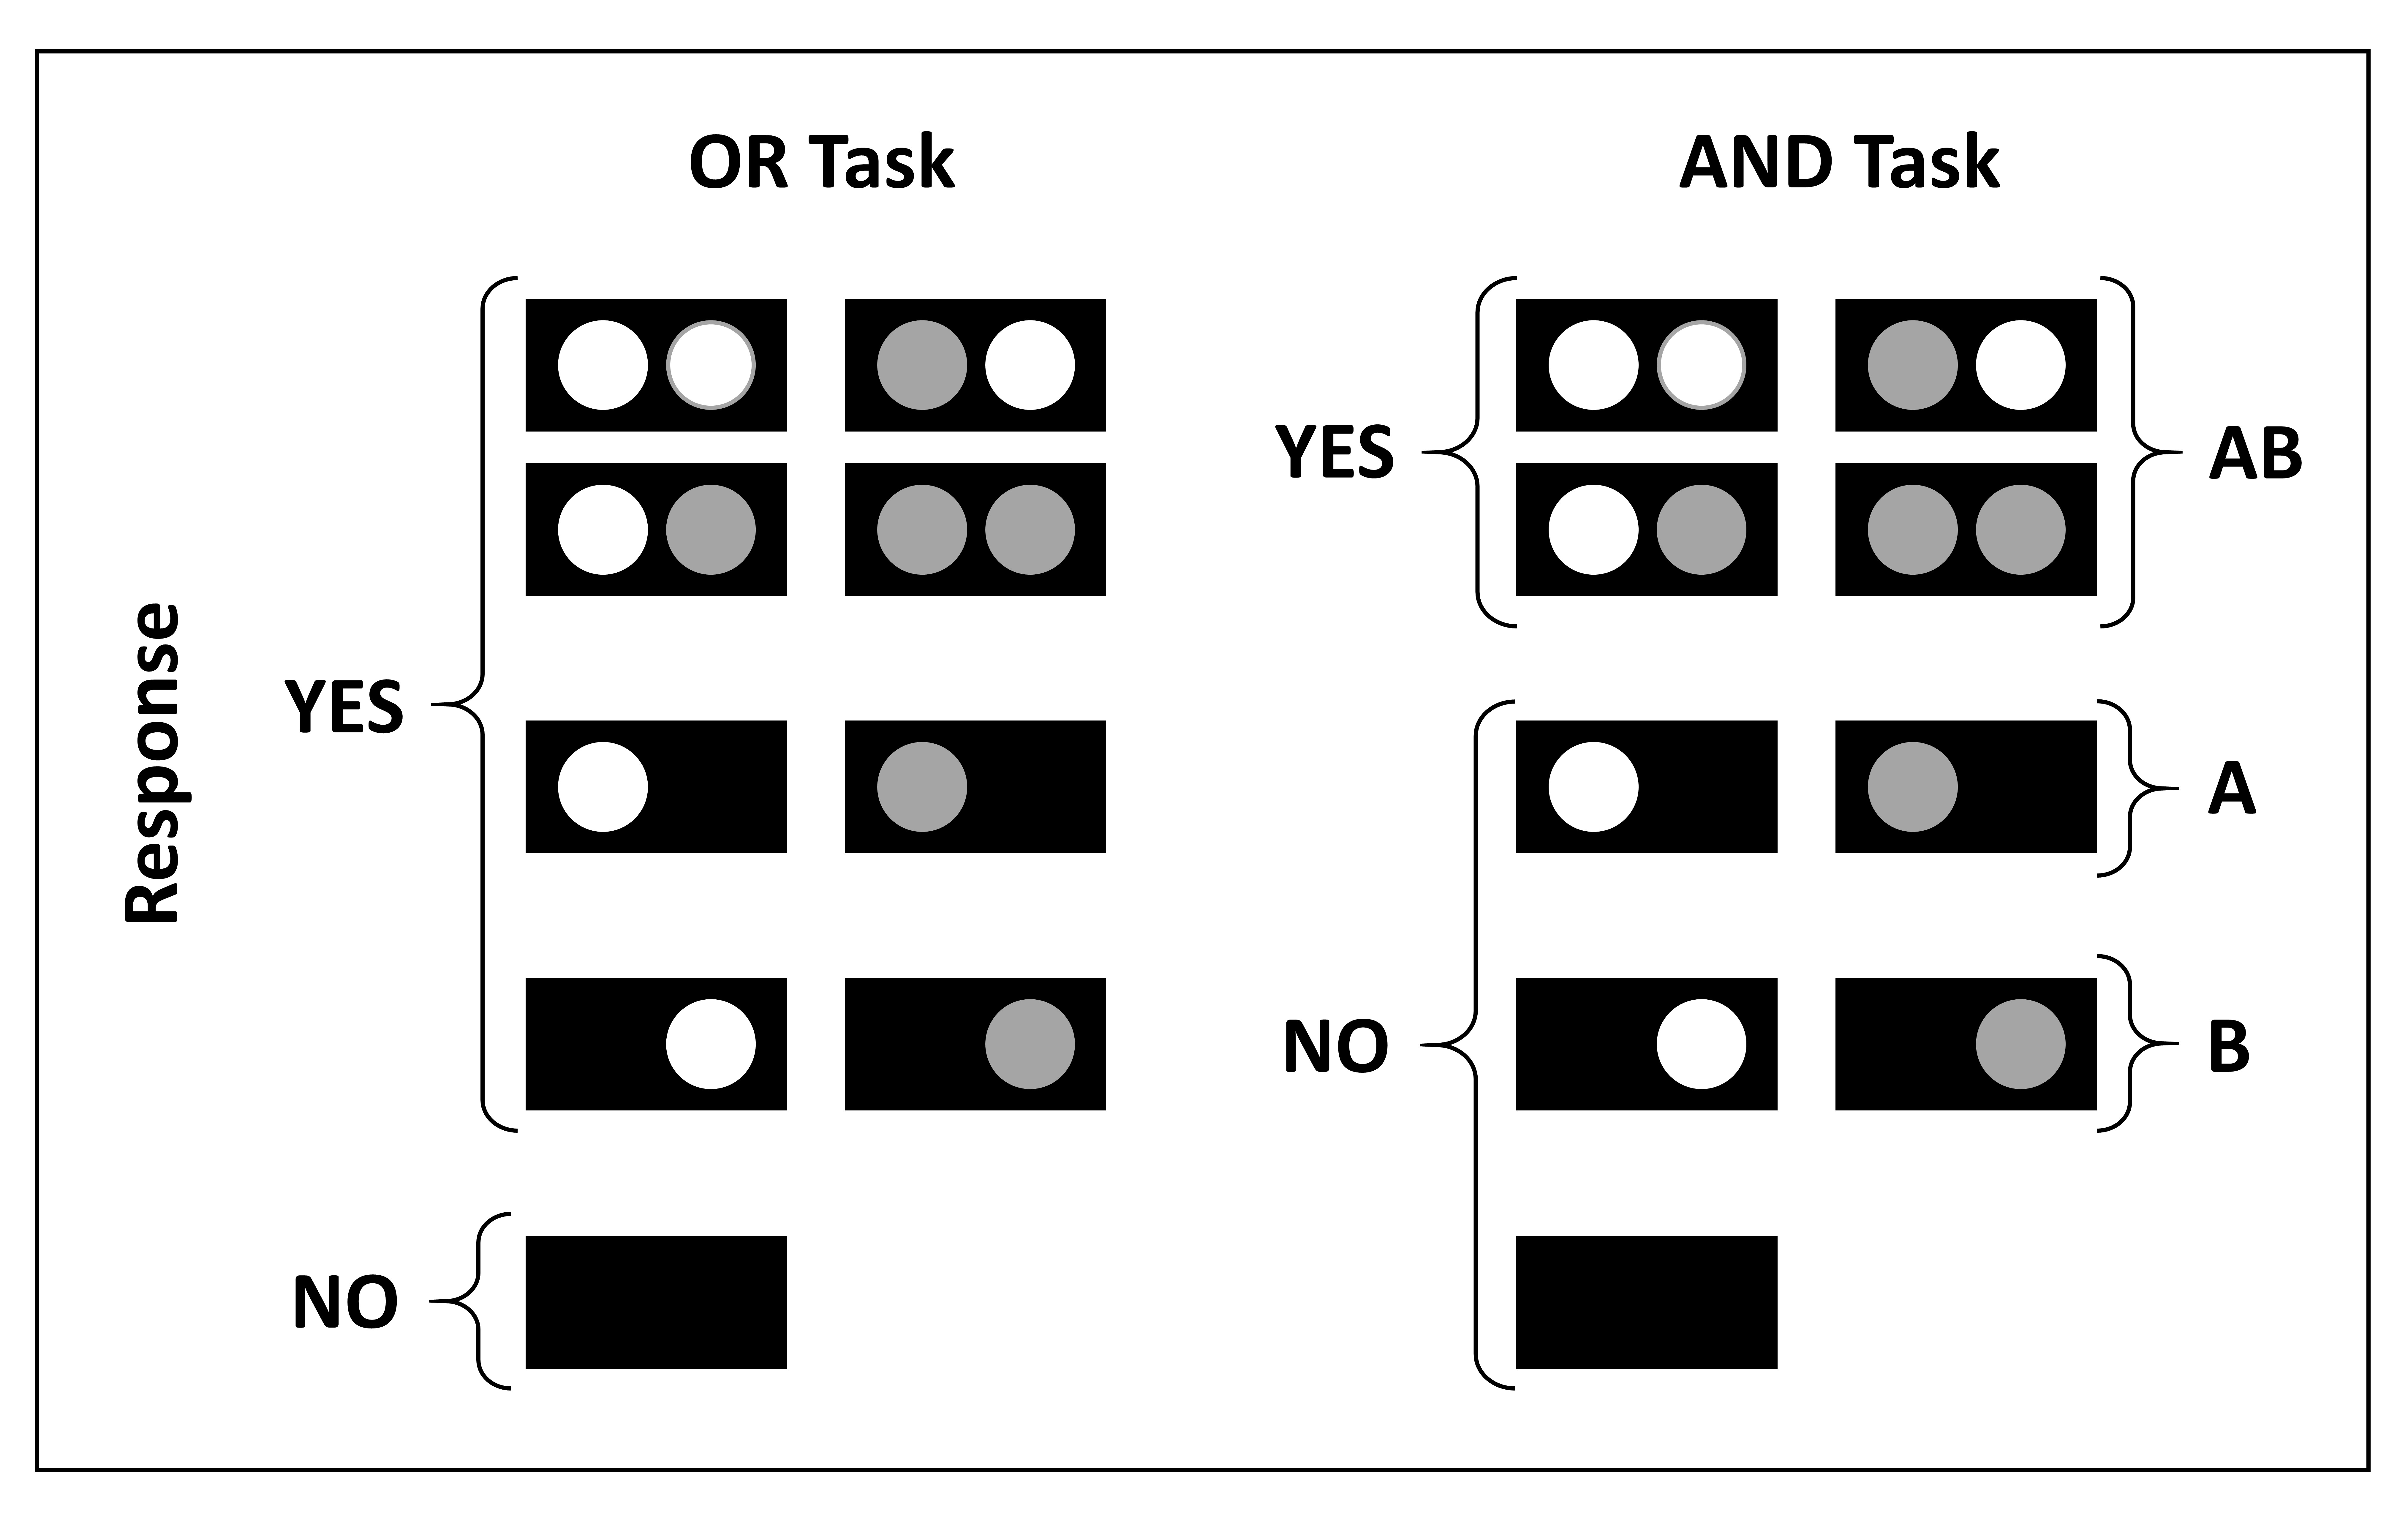
\includegraphics[scale=.6]{Figures/Mix/AndvsOR.jpg}
\caption{Stimuli from the classic redundant-target double-factorial paradigm of Townsend and Nozawa (1995), with responses mapped for an OR (left) and AND (right) task design. AB: double-target. A: single-target left. B: single-target right.}
\label{fig:Ch5_AndvsOR}
\end{figure}

\subsection{OR capacity}
In Chapter 1, we covered the capacity coefficient for an OR task. In an OR task, capacity is measured relative to the self-terminating (minimum-time) benchmark of unlimited capacity, independent-channel, parallel (UCIP) race-model. Under this model, double-target processing times are equal to the sum processing times of each target-channel in isolation. These processing times can be expressed in terms of their distribution over time using a survivor function. A survivor function [S($t$)] characterizes the probability of a process not-continuing by time $t$; it is calculated as one minus the cumulative distribution function [1 - F($t$)]. This can also be represented in terms of a cumulative hazard function [H($t$) = -$\log$ S($t$)]. Under the self-terminating UCIP model, the capacity coefficient compares double-target finishing times [H$_{AB}$($t$)] to the finishing times of each channel in isolation [H$_{A}$($t$), H$_{B}$($t$)] and may be expressed as:

\begin{equation}
	\rm C_{OR}(\t) = \frac{-\log[S_{AB}(\t)]}{-\log[S_{A}(\t)] - \log[S_{B}(\t)]}
    \label{eq:Cor}
\end{equation}

\subsection{AND capacity}
For an AND task, capacity is computed compared to the maximum time benchmark of the UCIP exhaustive model, (\ie the slowest processing channel times). This can be specified in terms of the reverse integrated hazard function, [\ie the logarithmic transformation of the cumulative distribution function, -$\log$F($t$)], for double-target processing channels, compared to the reverse integrated hazard function predicated by the maximum of each single-target processing channel. The AND capacity coefficient can be expressed as: 

\begin{equation}
    \rm C_{AND}(\t) = \frac{-\log[F_{A}(\t)]-\log[F_{B}(\t)]}{-\log[F_{AB}(\t)]}
    \label{eq:Cand}
\end{equation}

As the \Cor and \Cand are both calculated under the assumptions of a UCIP model, each under their respective self-terminating or exhaustive stopping-rules; interpretations remain the same between each function. An unlimited capacity system that is unaffected by additional processing channels, predicts C($t$) = 1. A limited capacity system that slows with additional processing channels, (\ie slower double-target trials), predicts C($t$) $<$ 1, and a super capacity system that speeds with additional processing channels, (\ie a coactive model), predicts C($t$) $>$ 1.

\section{Pure to mixture models}
Over the course of this thesis, much time has been dedicated to the assessment of system architecture using the SIC. As illustrated in Chapter 1, each combination of stopping-rule and processing architecture, predicts a qualitatively unique SIC($t$) function (see Figure \ref{fig:SIC}). Identifying these `pure' processing models in empirical data has been the primary aim of SFT, with many statistical tools being developed to aid this identification \cite{houpt2010statSIC, houpt2012statCap, houpt2017hierarchical, houpt2017bayesSIC, Houpt2016, Thiele2017}. While some efforts have been made to identify mixture models in empirical data \cite<see>{Little2011, Moneer2016, Cheng2018}, the canonical signatures of the SIC($t$) and C($t$) have not been established for these mixture processes. 

In the following section, we will systematically simulate the range of potential models for various combinations of processing architecture within both `OR' and `AND' task designs. We will then visualise these mixture models using the distributional response-time measures, the SIC($t$) and C($t$). We aim to provide a new set of canonical SIC($t$) and C($t$) predictions, with which mixture models can be identified.

\section{Simulations}
To simulate mixtures of processing architecture and capacity, started by simulating the five `canonical' system models: parallel self-terminating, serial self-terminating, parallel exhaustive, serial exhaustive and coactive. 

\color{\Red}
\subsection{Canonical models}
We simulated each of the independent processing channels of the serial and parallel models as well as a coactive models (where input from two channels is combined prior to decision) using pairs of Poisson accumulators, Linear Ballistic accumulators \cite<LBA;>{Brown2008} and random walk accumulators. Although theoretically different, these accumulators have two similar components: a rate parameter and a decision threshold parameter. The rate parameter dictates the rate evidence accumulates towards the decision threshold which, once crossed, terminates the accumulation process and yields a channel completion-time. %AE: discard >>> \footnote{The Poissson accumulator is a distribution of RTs rather than a sequential accumulation process, however, the basic principles needed to grasp channel RT in each processing model remains unchanged.}. 
Manipulation of the rate parameter simulates high and low salience conditions, given a fixed decision threshold. Finally, channel completion-times from each of the two accumulators are combined using the specific operational order and decision rules dictated by the generating system model.

% AE: for each channel separately i suggest to use completion time  (or processing) time -- but NOT response time, as individual channel do not emit a response
% PG: Yep, fixed. Thanks

Figure \ref{fig:Ch5_ProArch} illustrates the operational order and decision rules by which channels were combined and response-times (i.e., channel completion times) were simulated for double-target trials under each canonical processing model. Note that for coactive processing models we assumed complete cross-talk between the channels such that the coactive accumulator rate was equal to the summed rate of both single target accumulators \cite<see>{Johnson2010b}. Simulating single-target and double-target trials under these five canonical models, allows us to generate simulated SIC(\textit{t}) and C(\textit{t}) functions. 

\begin{figure}[htb]
\centering
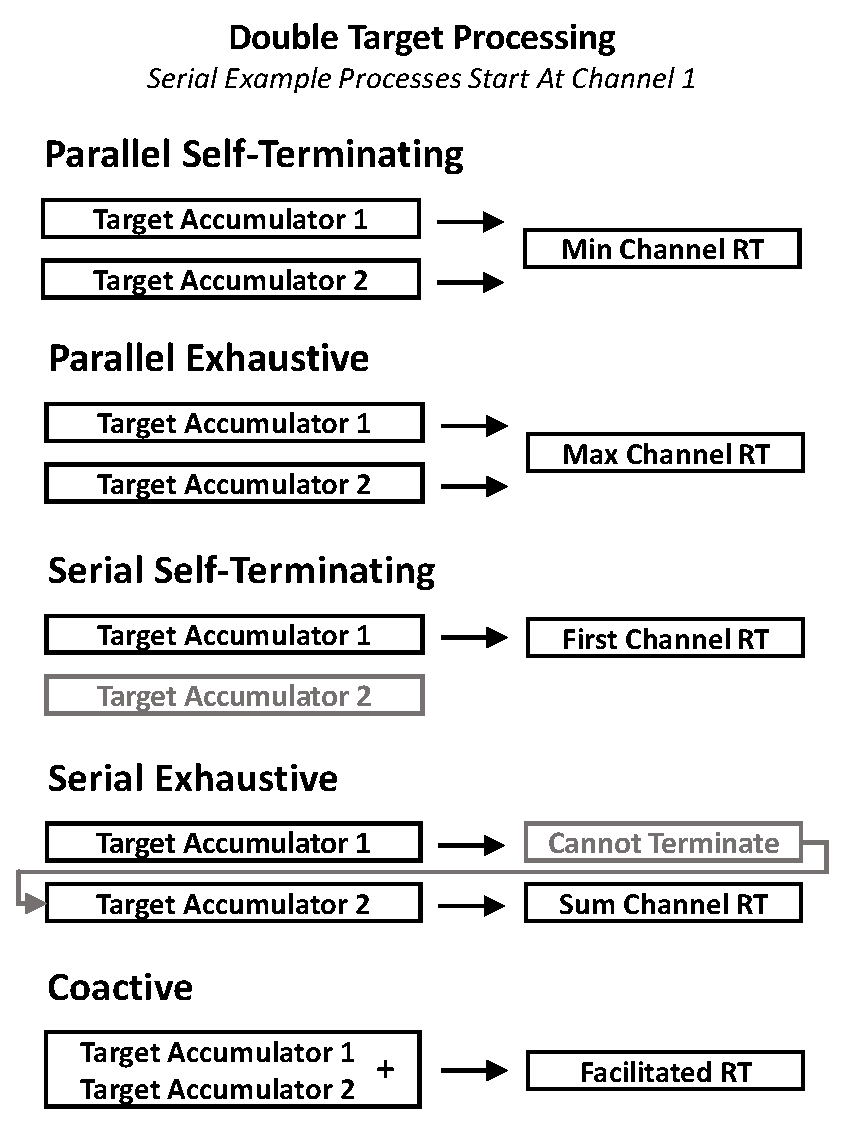
\includegraphics[scale = .85]{Figures/Mix/DoubleTargetProcessing.pdf}
\caption{Illustration of double-target channel operations used to simulate the five canonical processing models: parallel self-terminating, parallel exhaustive, serial self-terminating, serial exhaustive and coactive. Accumulators were either pairs of Poisson, linear ballistic or random walk accumulators. Single target channel RTs were simulated by their respective single accumulator.}
\label{fig:Ch5_ProArch}
\end{figure}

\color{black}

\subsection{Mixture models}
Mixture models were computed as the additive mixtures of the component canonical models, with $p$ the probability that the mixture model used a parallel process, and $1-p$ the probability that the mixture used another process (coactive or serial). While our modeling allowed for mixtures of architectures (serial, parallel, and coactive), it did \emph{not} allow for a mixtures across stopping-rules. For the OR decision rule, we used the parallel self-terminating model and the serial self-terminating model, and for the AND decision rule, we used the parallel exhaustive and serial exhaustive models. The stopping rule distinction does not apply to the coactive processing model.

Mixture models represent cases where across different trials the observer probabilistically adopts a different processing model. We simulated the predictions of the mixture models for the capacity coefficient and SIC with the probability of parallel processing, $p$, set to $0, .2, .4, .6, .8,$ or $1$. For all of the simulations, we used parameter values for which each channel produced distributions which had roughly the same mean RT, constraining the various canonical models to roughly the same time range. This constraint is driven by empirical observations.

When the means of the distributions diverge by a large extent, the functional predictions of each component SIC can become separated in time. For example, a negative parallel SIC might be followed by a serial SIC that produces a second negative component and then a positive component. Such a strong separation in the empirical data is yet to be witnessed \cite<\eg>{Little2011, Moneer2016}. We suspect this is because mixtures are unlikely when one component process is much less efficient than the other. As such, our simulated mixture models will focus exclusively on those instances where both mixture processing models are roughly equivalent in processing efficiency. 

\subsection{Poisson accumulator}
We simulated the completion times of each processing channel by a number of accumulated counts distributed as a Poisson random variable with a rate parameter $\lambda$ and a decision threshold parameter $a$. We use the subscripts 1 and 2 to indicate which of the two channel components of the model we are referring to. For all models, we set $a_1 = a_2 = 10$. For the capacity simulations, we set $\lambda_1 = \lambda_2 = .05$. For the SIC simulations, we set $\lambda_L = .02$ and $\lambda_H = .05$. Simulated processing-times were sampled from the relevant parallel model at a probability of $p$, and from the alternate model with a probability $1-p$. 

A benefit of the Poisson accumulator is that this analytic model is easily subjected to formal mathematical proofs. A formal mathematical description of the Possion accumulator for each processing channel is provided in the supplementary materials S3 (equations \ref{eq:poisspdf}--3). Formal proofs for each canonical processing model (equations \ref{eq:parst}--\ref{eq:serex}), each mixture model (equation \ref{eq:mixtures}), the capacity coefficient mixture process (equations \ref{eq:Fmix}--\ref{eq:CtMix}), and the SIC mixture process (equation \ref{eq:SICmix}) are all provided in supplementary materials S3. These proofs were used in the production of the following Poisson mixtures and are a formal expression of the processes illustrated in Figure \ref{fig:Ch5_ProArch}. For the purpose of exposition, these proofs will not be focused upon further and our simulated results will now be presented.

\subsubsection{Capacity predictions} 
The capacity predictions for two kinds of mixture models, parallel processing coupled with either serial or coactive processes, for both the OR and AND case, are shown in Figure~\ref{fig:Ch5_CapPoisson}. For the coactive/parallel mixture model, as $p$ increases from 0 to 1, the predictions clearly reflect a smooth transition from the unlimited capacity parallel model predictions to the supercapacity coactive model predictions. Conversely, for the parallel/serial mixture model, the capacity predictions move smoothly from unlimited to limited capacity. 

For both the OR and the AND capacity functions, the presence of any amount of coactivity causes changes in the limit behavior of the function. For \Cor the left limit increases sharply reflecting the increased rate of processing for the double target as smaller values of $t$ relative to the single targets. For the single targets, there is no difference between a coactive or a parallel process since there is by definition only a single source of information. Likewise, for the AND capacity there is an increase in the \Cand function for smaller values of $t$. The opposite effect arises for the mixture of serial and parallel processing. Again, for the single targets, there is no difference between the serial and parallel predictions, but introducing any proportion of serial processing into the mixture leads to a decrease in capacity at longer values of $t$. Note that when the process is completely serial, \Cor = .5 for all $t$ indicating limited, fixed capacity. 
 
\begin{figure}[htb]
\centering
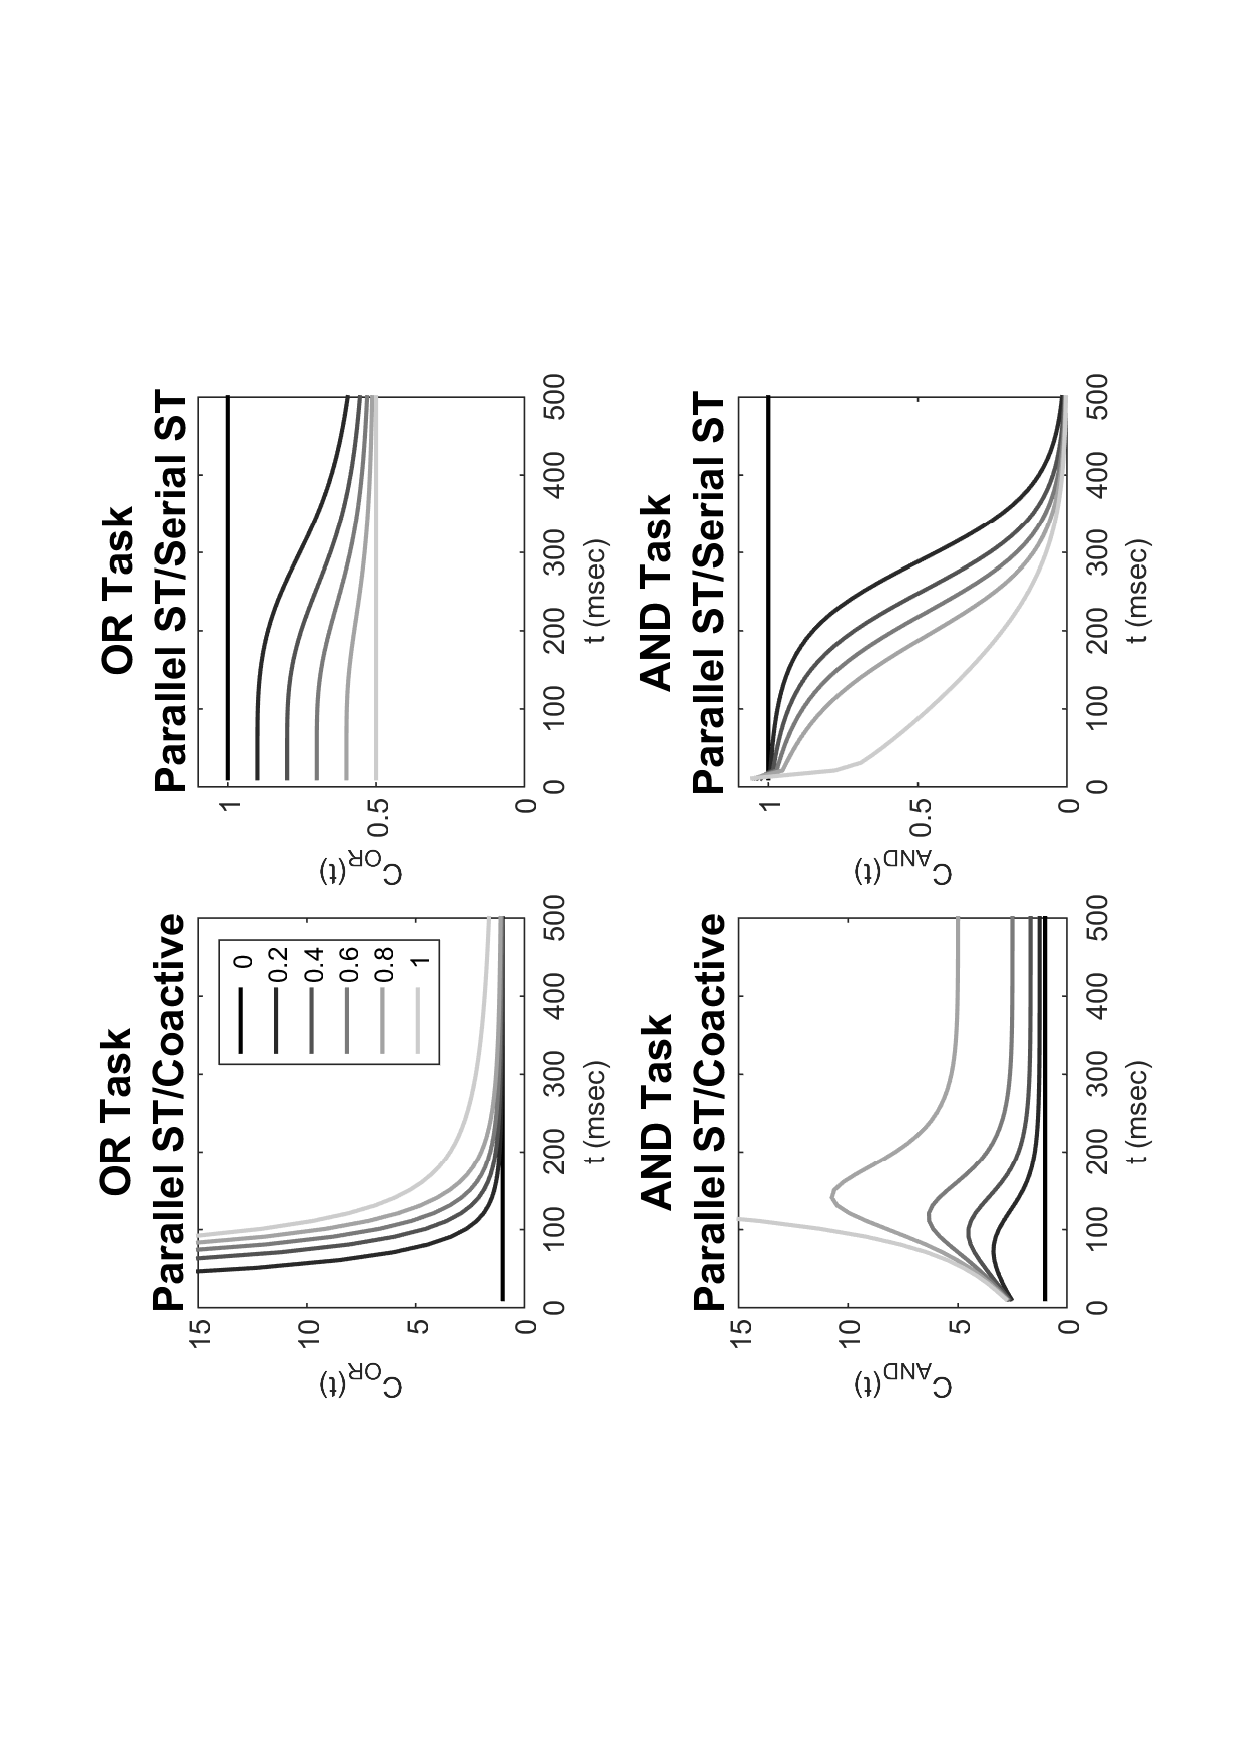
\includegraphics[scale=.7, angle=-90]{Figures/Mix/Figure_2.pdf}
\caption{Top: OR capacity coefficient predictions for the coactive/parallel self-terminating (left) and serial/parallel self-terminating (right) mixture models. Bottom: AND capacity coefficient predictions for the parallel exhaustive/coactive (left) and parallel exhaustive/serial exhaustive (right) mixture models. Simulations of each component process were instantiated as a pair of Poisson accumulators.}
\label{fig:Ch5_CapPoisson}
\end{figure}


\subsubsection{SIC predictions} 
The SIC predictions for the mixture models are shown in Figure~\ref{fig:Ch5_SICpoisson}. Like the capacity predictions, both sets of predictions transition smoothly between the parallel predictions and coactive or serial predictions for the parallel/coactive and parallel/serial models, respectively. 

\begin{figure}[htb]
\centering
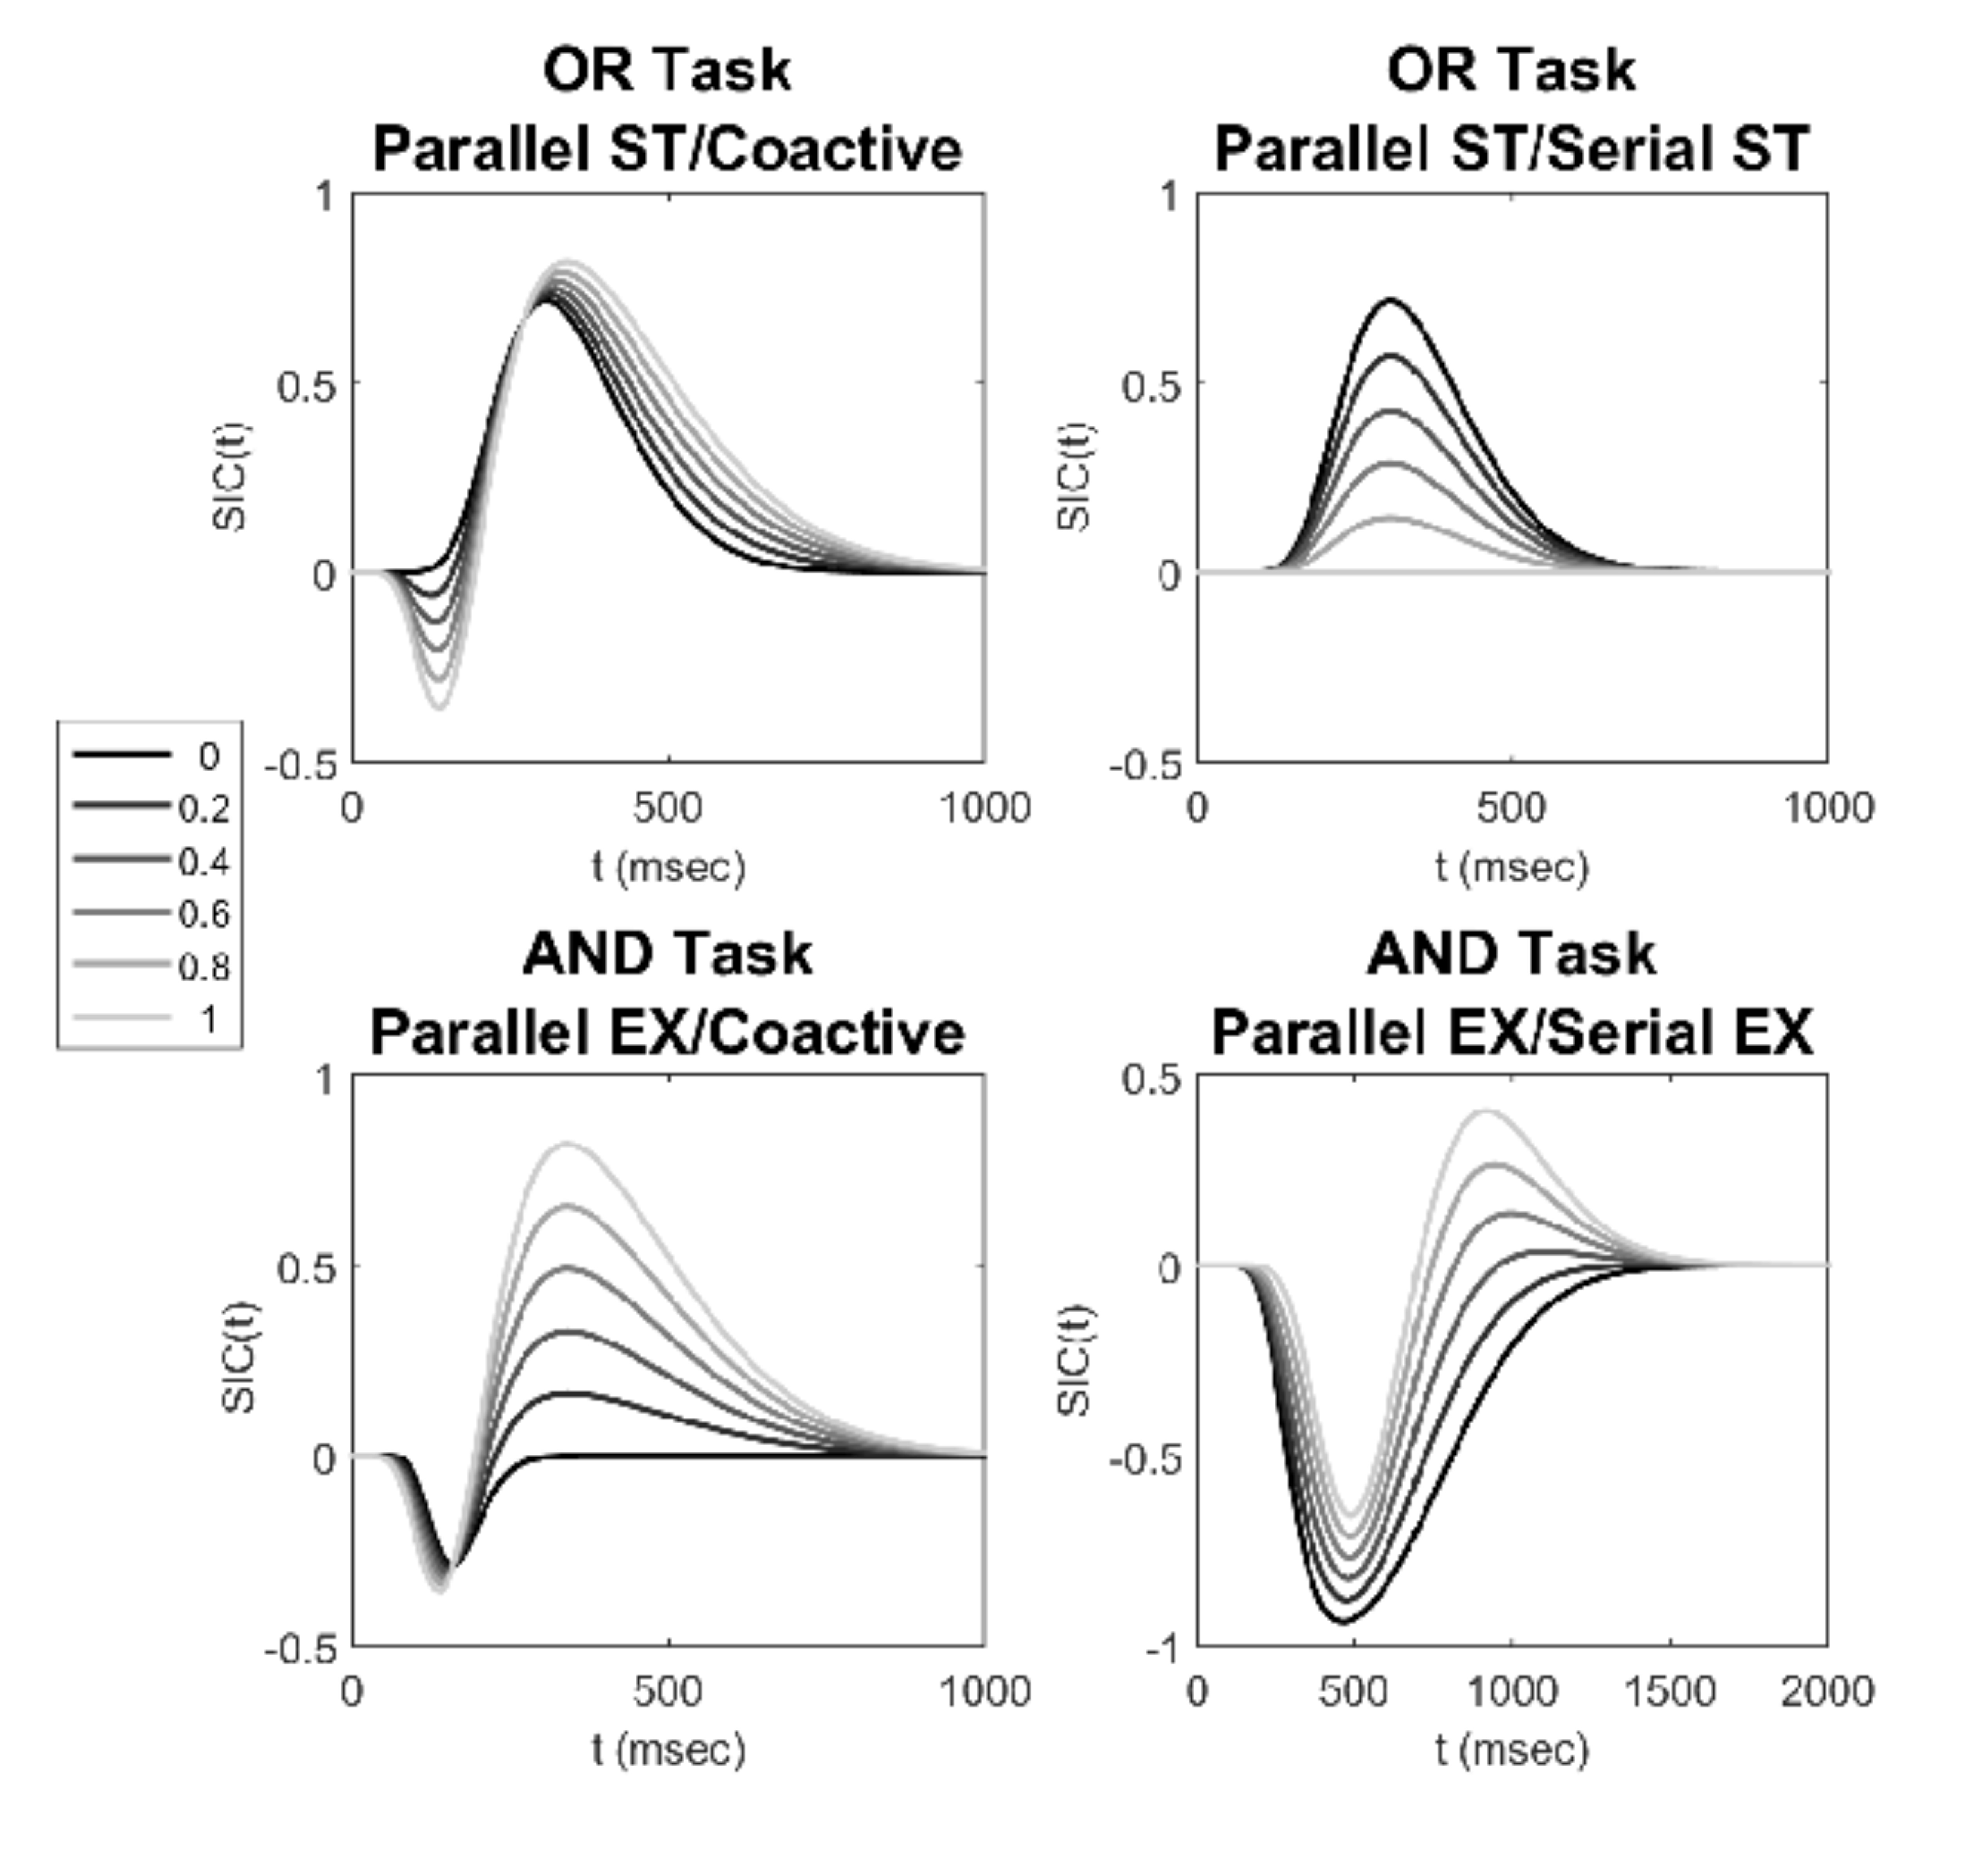
\includegraphics[scale=1]{Figures/Mix/SICpoisson.jpg}
\caption{Top: survivor interaction contrast (SIC) predictions for the self-terminating coactive/parallel (left) and self-terminating serial/parallel (right) mixture models. Bottom: survivor interaction contrast (SIC) predictions for the exhaustive coactive/parallel (left) and exhaustive serial/parallel (right) mixture models. Simulations of each component process were instantiated as a pair of Poisson accumulators.}
\label{fig:Ch5_SICpoisson}
\end{figure}


\subsection{Interim summary}
Mixing serial, parallel, and coactive processes results in a wide range of SFT signatures that go well beyond the canonical signatures initially studied by \citeA{Townsend_1995}. Relaxing the assumption that responses on all trials in an experiment are homogeneous (though stochastic) and come from a single process by combining processes from different distributions with different mixture-probabilities, allows a fair amount of flexibility in the predicted signature. This flexibility is also reflected in the simulated behavioral outcomes, as measured by \SIC and \Ct which change with the mixing proportion $p$. Thus, instead of a unique and well-defined SIC signature for a parallel model (say, positive for all time $t$), a mixture of parallel and coactive processes could predict anything between an all-positive SIC to a partly-negative SIC (for early $t$) to a partly-positive SIC (for longer $t$), as shown in the top left panel of Figure~\ref{fig:Ch5_SICpoisson}. 

Importantly, our mixture model simulations reveal that changes to the \SIC and C(\textit{t}) are completely \textit{predictable} (as suggested informally by \citeNP{Fific2008}, and later by \citeNP{TillmanStopping}). That is, the \SIC and \Ct signatures of probability mixtures are bounded between the extreme signatures defined by $p$=0 and $p$=1. Moreover, within these bounds they change in a predictable and systematic way, looking similar to parallel signature for small $p$, and gradually taking the form of the alternate component in the mixture as $p$ increases. To further validate our findings, we extended the scope of our simulations, and simulated these mixture models with different underlying processes.

\subsection{Computation simulations: LBA}
We simulated the mixture model results under the assumption that each channel was an independent linear ballistic accumulator, with an error drift rate set to zero. Each of the accumulator processes is characterized by the following parameters: drift rate $\nu_i$, for each of the simulated channels $i$, a response threshold, $b$, the width of the uniform starting point distribution, $A$, and the standard deviation of the normal drift distribution representing between trial variability, $s$. Response thresholds were set to 3, starting point variability was set to 2 and the standard deviation of the drift was set to 1. The non-decision time parameter, $Ter$, was set to 0. Drift rates for each model for the SIC and capacity coefficient simulations are shown in Table \ref{tab:lba_drifts}. 

\begin{table}[htb]
\centering
\caption{Drift rates for each stimulus component and their combination (Coactive) or individual stimulus component (Serial \& Parallel) for SIC and capacity coefficient mixtures. We use the A \& B values to simulate SIC($t$)$_{OR}$ functions, and X \& Y values to simulate SIC($t$)$_{AND}$ functions. Subscripts $h$ and $l$ refer to the salience of each channel. Coactive drift rates were identical for both OR and AND functions.}
\begin{tabular}{l l l l r r } 
\hline
Stimulus & Coactive   		& ~ & Stimulus   &  Serial 	& Parallel 	\\
\hline
$A_hB_h$ & 10.8             & ~ & $A_h$      & 7         & 7         \\
$A_hB_l$ & 6.8              & ~ & $A_l$      & 3         & 3         \\
$A_lB_h$ & 6.8              & ~ & $B_h$      & 7         & 7         \\
$A_lB_l$ & 2.8              & ~ & $B_l$      & 3         & 3         \\
$X_hY_h$ & 10.8             & ~ & $X_h$      & 7         & 7         \\
$X_hY_l$ & 6.8              & ~ & $X_l$      & 3         & 3         \\
$X_lY_h$ & 6.8              & ~ & $Y_h$      & 7         & 7         \\
$X_lY_l$ & 2.8              & ~ & $Y_l$      & 3         & 3    
\\
\hline
\hline
\label{tab:lba_drifts}
\end{tabular} 
\end{table}

To simulate the coactive LBA model, complete cross-talk between the processing channels was assumed, such that sharing the probability of a single count was always 1. Predictions for the coactive model were simulated by summing the drift rates sampled from two independent channels, $\nu_{1}$ and $\nu_{2}$. The drift rate for each independent channel was sampled from a normal distribution, centered on $\nu_i$, with standard deviation $s$. For each stimulus, 1 million RTs were simulated; RT predictions were binned by 5 msec ranging from 0 to 2,000 msec.

For the remaining models, individual channels were combined using equations quantitatively identical to the analytic proofs located in supplementary material S3, Equations~\ref{eq:parst}-\ref{eq:serex}. The results of these simulations are shown in Figures \ref{fig:capLBAmixture} and \ref{fig:sicLBAmixture}. To generate comparable mean RTs, the threshold and starting point parameters were decreased to 1.75 and 1.3 respectively, for parallel exhaustive models in the comparison of coactive and parallel exhaustive mixtures, and for serial exhaustive models in the comparison of serial and parallel exhaustive mixtures.

\begin{figure}[htb]
\centering
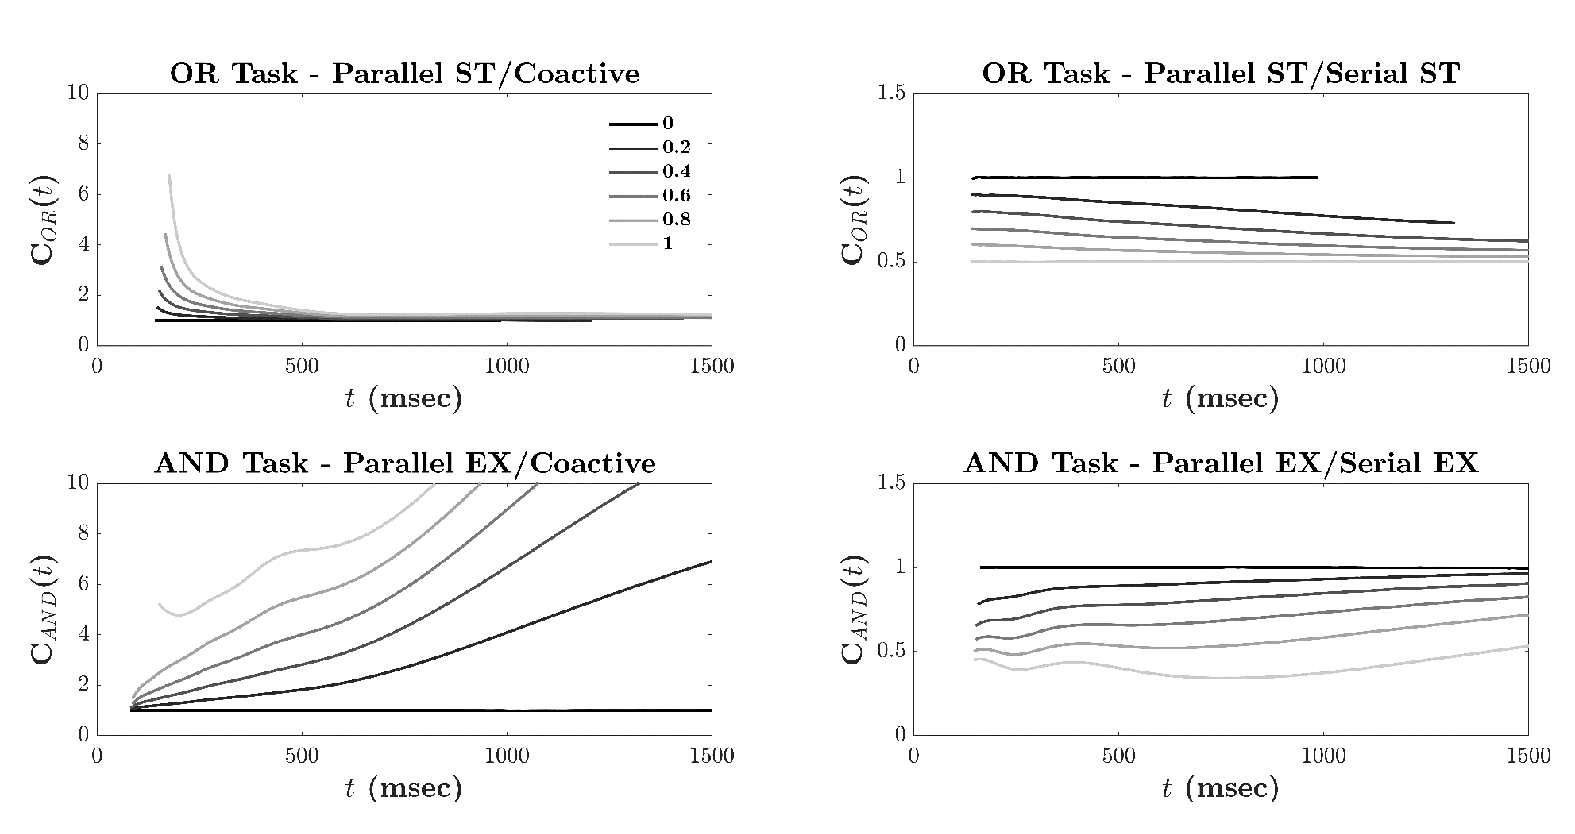
\includegraphics[scale=.6]{Figures/Mix/Figure_B1v3.pdf}
\caption{Linear ballistic accumulator predictions. Top: OR capacity coefficient predictions for the coactive/parallel (left) and serial/parallel (right) mixture models. Bottom: AND capacity coefficient predictions for the parallel/coactive (left) and parallel/serial (right) mixture models.}
\label{fig:capLBAmixture}
\end{figure}

\begin{figure}[htb]
\centering
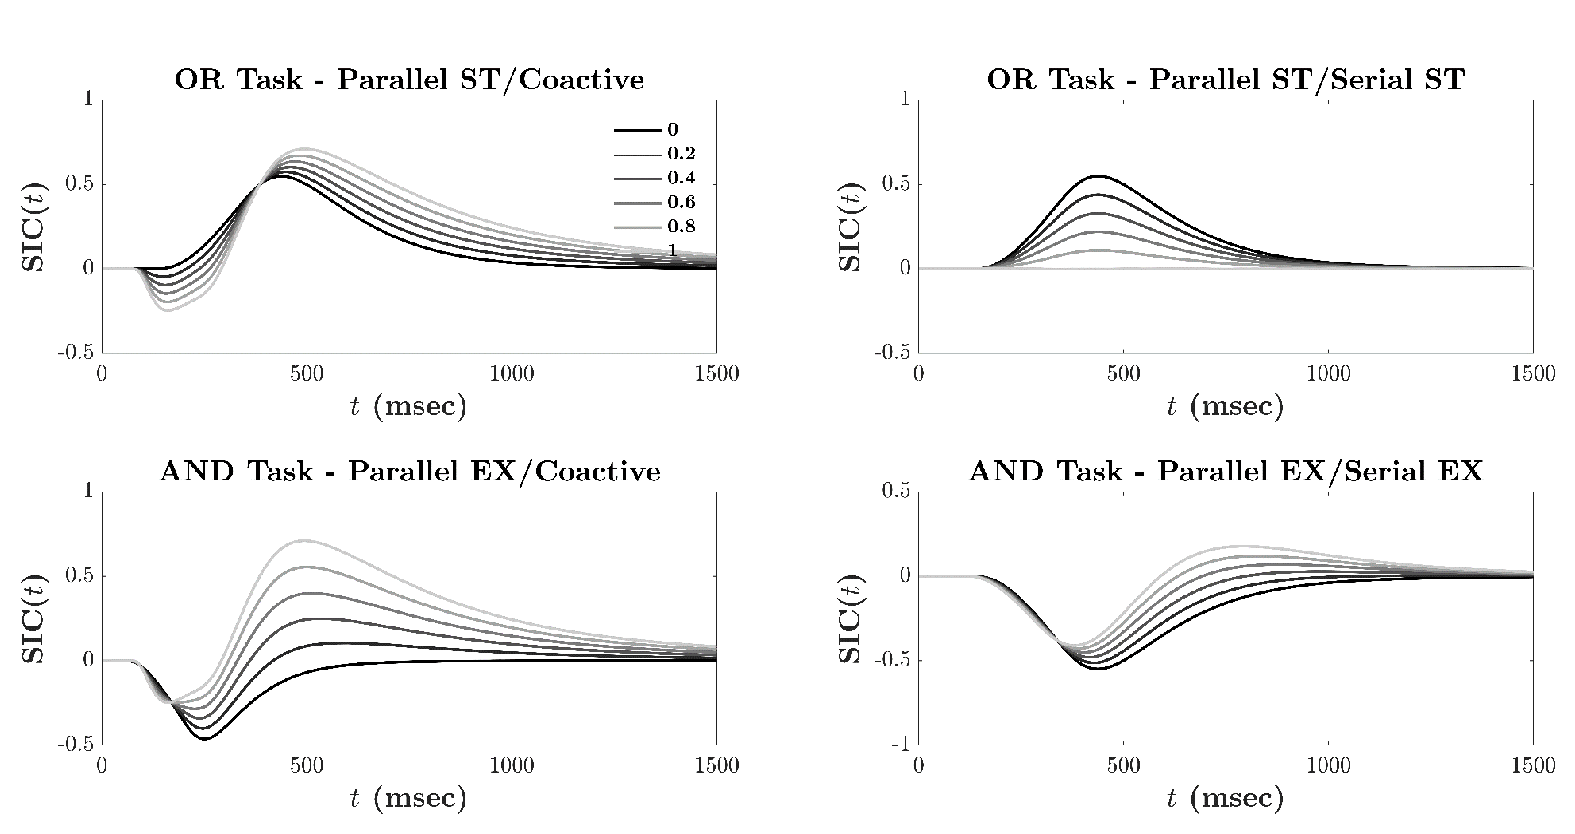
\includegraphics[scale=.6]{Figures/Mix/Figure_B2.pdf}
\caption{Linear ballistic accumulator predictions. Top: survivor interaction contrast (SIC) predictions for the self-terminating coactive/parallel (left) and self-terminating serial/parallel (right) mixture models. Bottom: survivor interaction contrast (SIC) predictions for the exhaustive coactive/parallel (left) and exhaustive serial/parallel (right) mixture models.}
\label{fig:sicLBAmixture}
\end{figure}


\subsection{Computation simulations: random walk}
We simulated the mixture model results under the assumption that each channel was a random walk. Each random walk is characterized by the following parameters: step rate $\nu_i$, where $\nu$ represents the rate at which discrete steps are sampled for each of the simulated channels $i$, threshold $a$ and bias $\beta$. Bias was kept constant at 0 for all simulations and target channel and error thresholds was set to 115 and -115, respectively.

Each step of the random walk was a discrete value of 1 or -1, with steps accumulating towards the upper or lower response threshold. Step rate $\nu$ of the random walk was a probability bound between 0 $\leq \nu \leq$ 1, with $\nu$ less than 0.5 increasing the rate at which negative steps were sampled, and $\nu$ greater than 0.5 increasing the rate at which positive steps were sampled. The non-decision time parameter, $T$er was set to 0. We adopted this assumption since we are primarily interested in mixtures of the decision stage of processing; however, it must be acknowledged that manipulations of salience may also affect non-decision processes like encoding. Step probabilities for each model in the SIC and capacity coefficient simulations are shown in Table~\ref{tab:RW_drifts}. 

\begin{table}[tbh]
\centering
\caption{Random walk step probabilities, reported in terms of $\nu$, for each stimulus component and their combination (Coactive) or individual stimulus component (Serial \& Parallel) for SIC and capacity coefficient mixtures. We use the A \& B values to simulate the SIC($t$)$_{OR}$ function and the X \& Y values to simulate the SIC($t$)$_{AND}$ function. The subscripts $h$ and $l$ refer to the salience of the channel.}
\begin{tabular}{l l c l c c } 
\hline
Stimulus & Coactive   	   & ~ & Stimulus   &  Serial 	  & Parallel 	\\
\hline
$A_h$ &     .64            & ~ & $A_h$      & .685        & .685        \\
$A_l$ &     .57            & ~ & $A_l$      & .63         & .63         \\
$B_h$ &     .64            & ~ & $B_h$      & .685        & .685        \\
$B_l$ &     .57            & ~ & $B_l$      & .63         & .63         \\
$X_h$ &     .64            & ~ & $X_h$      & .685        & .685        \\
$X_l$ &     .57            & ~ & $X_l$      & .63         & .63         \\
$Y_h$ &     .64            & ~ & $Y_h$      & .685        & .685        \\
$Y_l$ &     .57            & ~ & $Y_l$      & .63         & .63         \\
$A_hB_h$ &  $A_h$ + $B_h$  & ~ &   ~        & ~           & ~           \\
$A_hB_l$ &  $A_h$ + $B_l$  & ~ &   ~        & ~           & ~           \\
$A_lB_h$ &  $A_l$ + $B_h$  & ~ &   ~        & ~           & ~           \\
$A_lB_l$ &  $A_l$ + $B_l$  & ~ &   ~        & ~           & ~           \\
$X_hY_h$ &  $X_h$ + $Y_h$  & ~ &   ~        & ~           & ~           \\
$X_hY_l$ &  $X_h$ + $Y_l$  & ~ &   ~        & ~           & ~           \\
$X_lY_h$ &  $X_l$ + $Y_h$  & ~ &   ~        & ~           & ~           \\
$X_lY_l$ &  $X_l$ + $Y_l$  & ~ &   ~        & ~           & ~           \\
\hline
\hline
\label{tab:RW_drifts}
\end{tabular} 
\end{table}

\subsubsection {Coactive random walk model} To simulate the coactive random walk model, complete cross-talk between processing channels was assumed. Predictions for the coactive model were simulated by summing the the two independent accumulator channels, $\nu_{1k}$ and $\nu_{2k}$, at each step of the independent random walks, $k$. This is shown in Table~\ref{tab:RW_drifts} by the summation of the terms. For each stimulus, 100,000 RTs were simulated; RT predictions were binned by 5 msec ranging from 0 to 2,000 msec.

For the remaining models, individual channels were combined using the same procedures as the LBA and Poisson models. The results of these simulations are shown in Figures \ref{fig:capRWmixture} and \ref{fig:sicRWmixture}. To generate comparable mean RTs, the threshold parameter was decreased to 67 for parallel exhaustive models in the comparison of coactive and parallel exhaustive mixtures; and for serial exhaustive models in the comparison of serial exhaustive and parallel exhaustive mixtures.

\begin{figure}
\centering
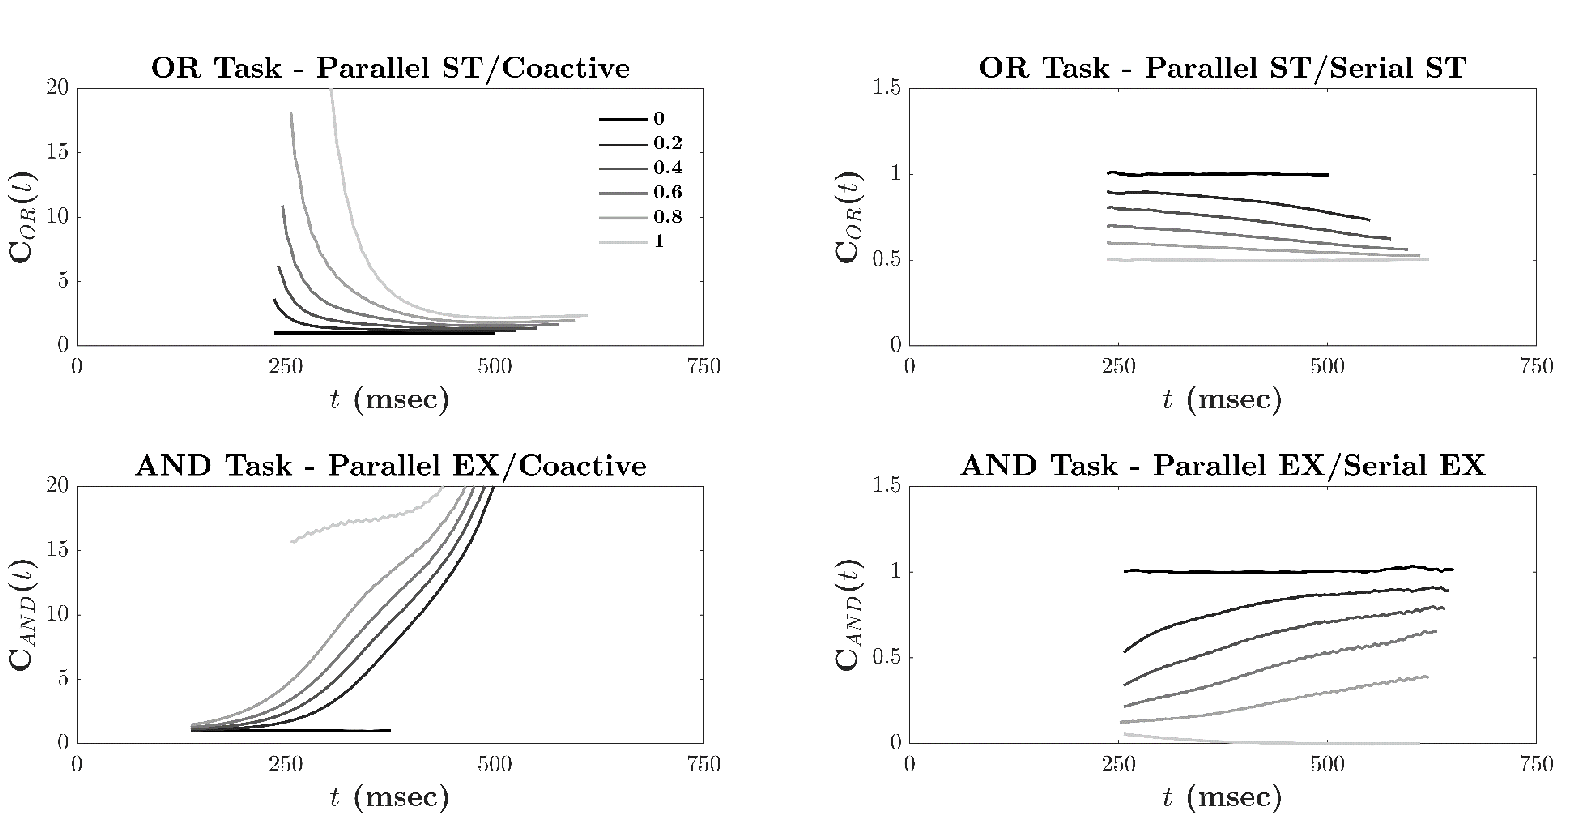
\includegraphics[scale=.6]{Figures/Mix/Figure_C1.pdf}
\caption{Random walk accumulator predictions. Top: OR capacity coefficient predictions for the coactive/parallel (left) and serial/parallel (right) mixture models. Bottom: AND capacity coefficient predictions for the parallel/coactive (left) and parallel/serial (right) mixture models.}
\label{fig:capRWmixture}
\end{figure}

\begin{figure}
\centering
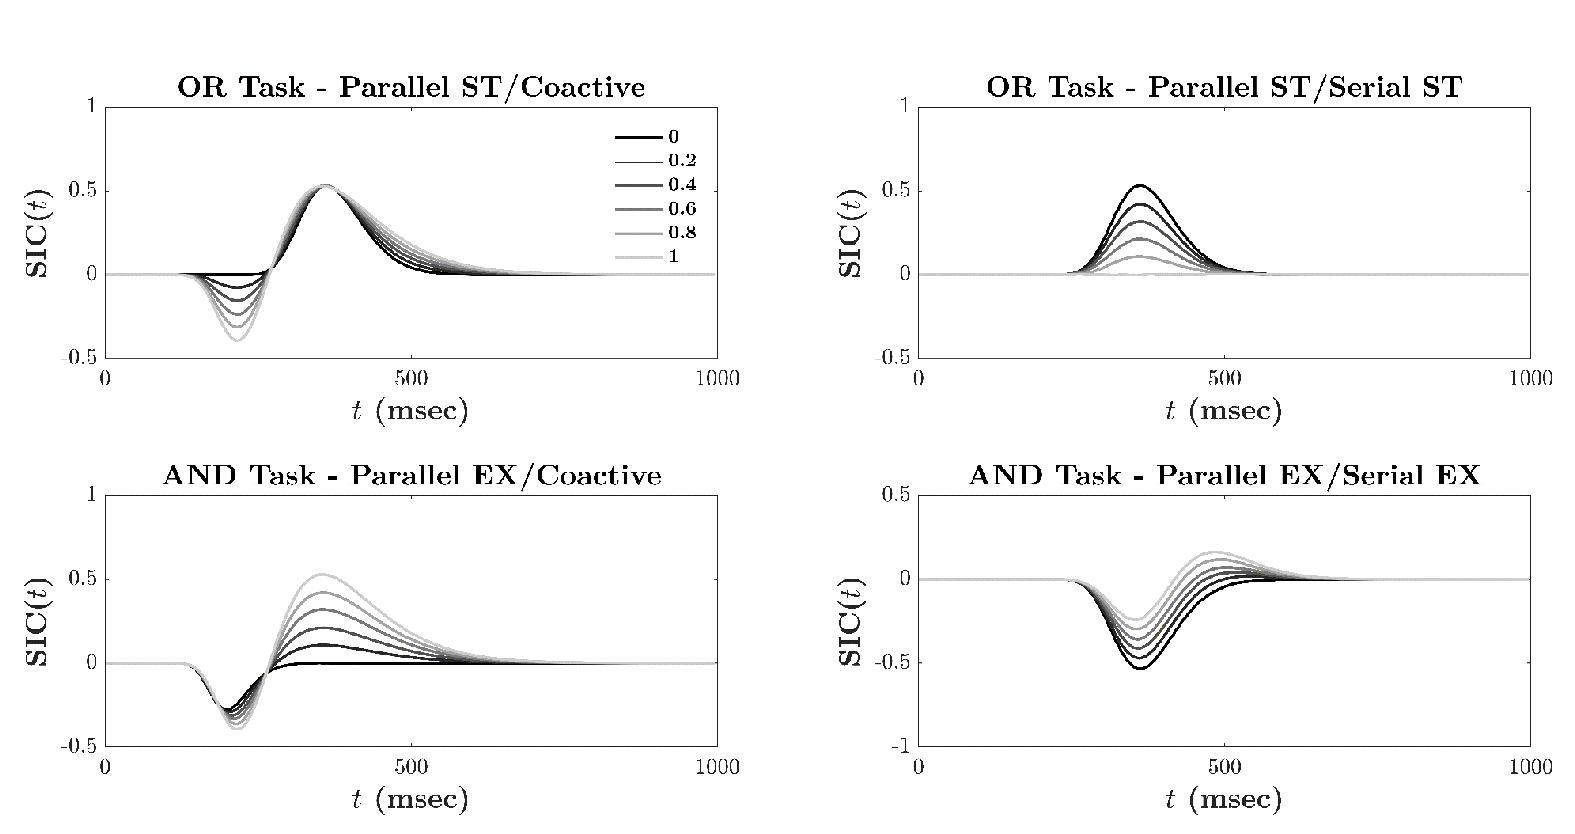
\includegraphics[scale=.6]{Figures/Mix/Figure_C2.pdf}
\caption{Random walk accumulator predictions. Top: survivor interaction contrast (SIC) predictions for the self-terminating coactive/parallel (left) and self-terminating serial/parallel (right) mixture models. Bottom: survivor interaction contrast (SIC) predictions for the exhaustive coactive/parallel (left) and exhaustive serial/parallel (right) mixture models.}
\label{fig:sicRWmixture}
\end{figure}


\section{Discussion}
% General Findings
The current investigation systematically varied the relative proportions of component `pure' system models, and visualized the SIC($t$) and C($t$) signatures of the simulated mixture models. In line with expectations \cite<e.g.,>{TillmanStopping, eidels2011}, SIC($t$) and C($t$) functions changed in predictable and systematic ways. Distributional signatures aligned with parallel model predictions when mixture proportions were zero, and smoothly transitioned to the predictions of the alternative model. At all time points, the mixture model signatures were bounded between the predictions of the two pure component models. These findings were shown to hold across three methods of computational simulation: Poisson, LBA and random-walk accumulators. 

\color{\Red}
% Subitizing Mixtures
Mixture model results from the current Chapter can be applied to the findings of Chapters 3 and 4. In the previous Chapter, we presented SIC($t$) functions that did not match the predictions of any single `pure' processing model (see Figure \ref{fig:subSICmix}). In one instance, we speculated these signatures might reflect the mixture of a parallel self-terminating and coactive processing model, and in another instance, a mixture of a parallel exhaustive and serial exhaustive processing models. Visual comparison of the empirical signatures to the simulated mixture models suggests participants deviated from the primary parallel system model, for approximately 10--20$\%$ of responses. Yet, relying only on visual inspection for identifying mixture models has clear limits.

Statistical tests have been previously developed for the identification of `pure' processing models \cite{houpt2010statSIC, houpt2012statCap, houpt2017hierarchical, houpt2017bayesSIC, Houpt2016, Thiele2017}, however, such tools do not yet exist to identify mixture models. Previous work has applied parametric techniques, such as computational modelling, to identify mixture processing models \cite{Little2011, Moneer2016, Cheng2018}; yet, these methods lack the strong non-parametric appeal that underlies SFT. The current work shows such methods can be supplemented by visual inspection of non-parametric measures, the SIC($t$) and C($t$). Further development of non-parametric methods for mixture model identification, (\ie statistical tools), is outside the scope of the current Chapter. We leave this as a challenge for future researchers.

\subsection{Conclusions}
The purpose of the current Chapter was to extend SFT beyond the canonical predictions of `pure' serial, parallel, and coactive architectures. We investigated SFT predictions for cases in which processing architecture could change on a trial-by-trial basis, resulting in probability mixtures of pure processing models. The SFT predictions for mixtures models follow intuitive expectations and allows for visual identification of non-canonical SIC($t$) and C($t$) patterns. This work extend SFT assessments of processing architecture and capacity beyond the scope of the canonical models. This work also allows previously developed parametric methods to benefit by considering our new mixture \SIC and \Ct functions when diagnosing mixture processes. The conclusion of this Chapter also represents the conclusion of that first research stream, that which focused upon the comparison of quantity. Now, we may progress to our second research stream and the confusion of numbers.
\color{black}

%%AE DONE 31/10/2019